\section{Another planetary defense mission: 2016 HO3}
\label{sec:7}

This section introduces another scientific mission, which interests people for its particularitiy. (469219) Kamo‘oalewa, provisionally designated 2016 HO3, is a quasi-satellite of the Earth, i.e. the asteroid stays always close to the Earth but it is orbiting around the Sun. It was discovered on April 27, 2016 by the Pan-STARRS program at the Haleakala observatory on the Hawaiian island of Maui. Its main specificity is its fast revolution period of 20 minutes. Studying this asteroid is relevant to understand the impact of its revolution period on its temperature.

\begin{center}
    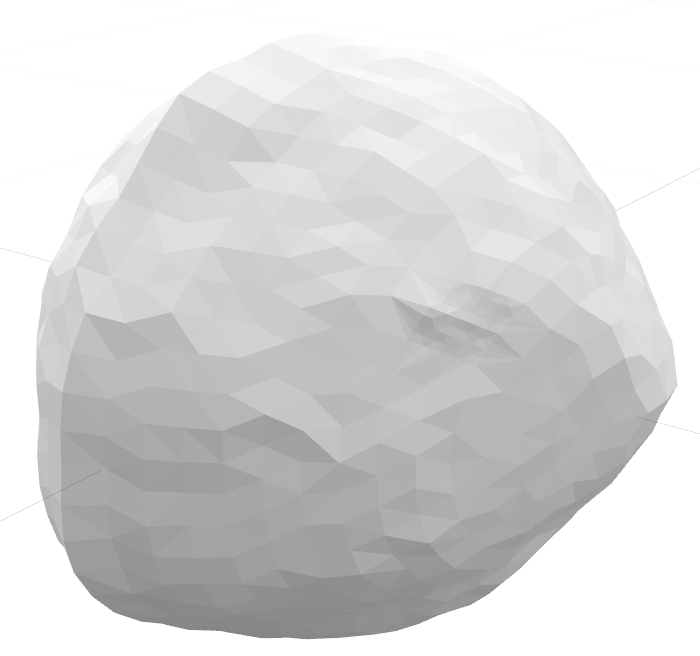
\includegraphics[width=0.6\linewidth]{rsc/HO3_shapemodel.png}
    \captionof{figure}{The shape model of the asteroid Bennu has been taken for simulations as there is no shape model yet for HO3 and both look alike. The asteroid HO3 as a mean radius of 20 meters, which makes it a very small asteroid.}
    \label{fig:7.1}
\end{center}

The shape model of Bennu has been resized to fit the dimensions of HO3. To get a clearer grasp, it is interesting to compare two thermal maps with different revolution periods. 

\begin{center}
    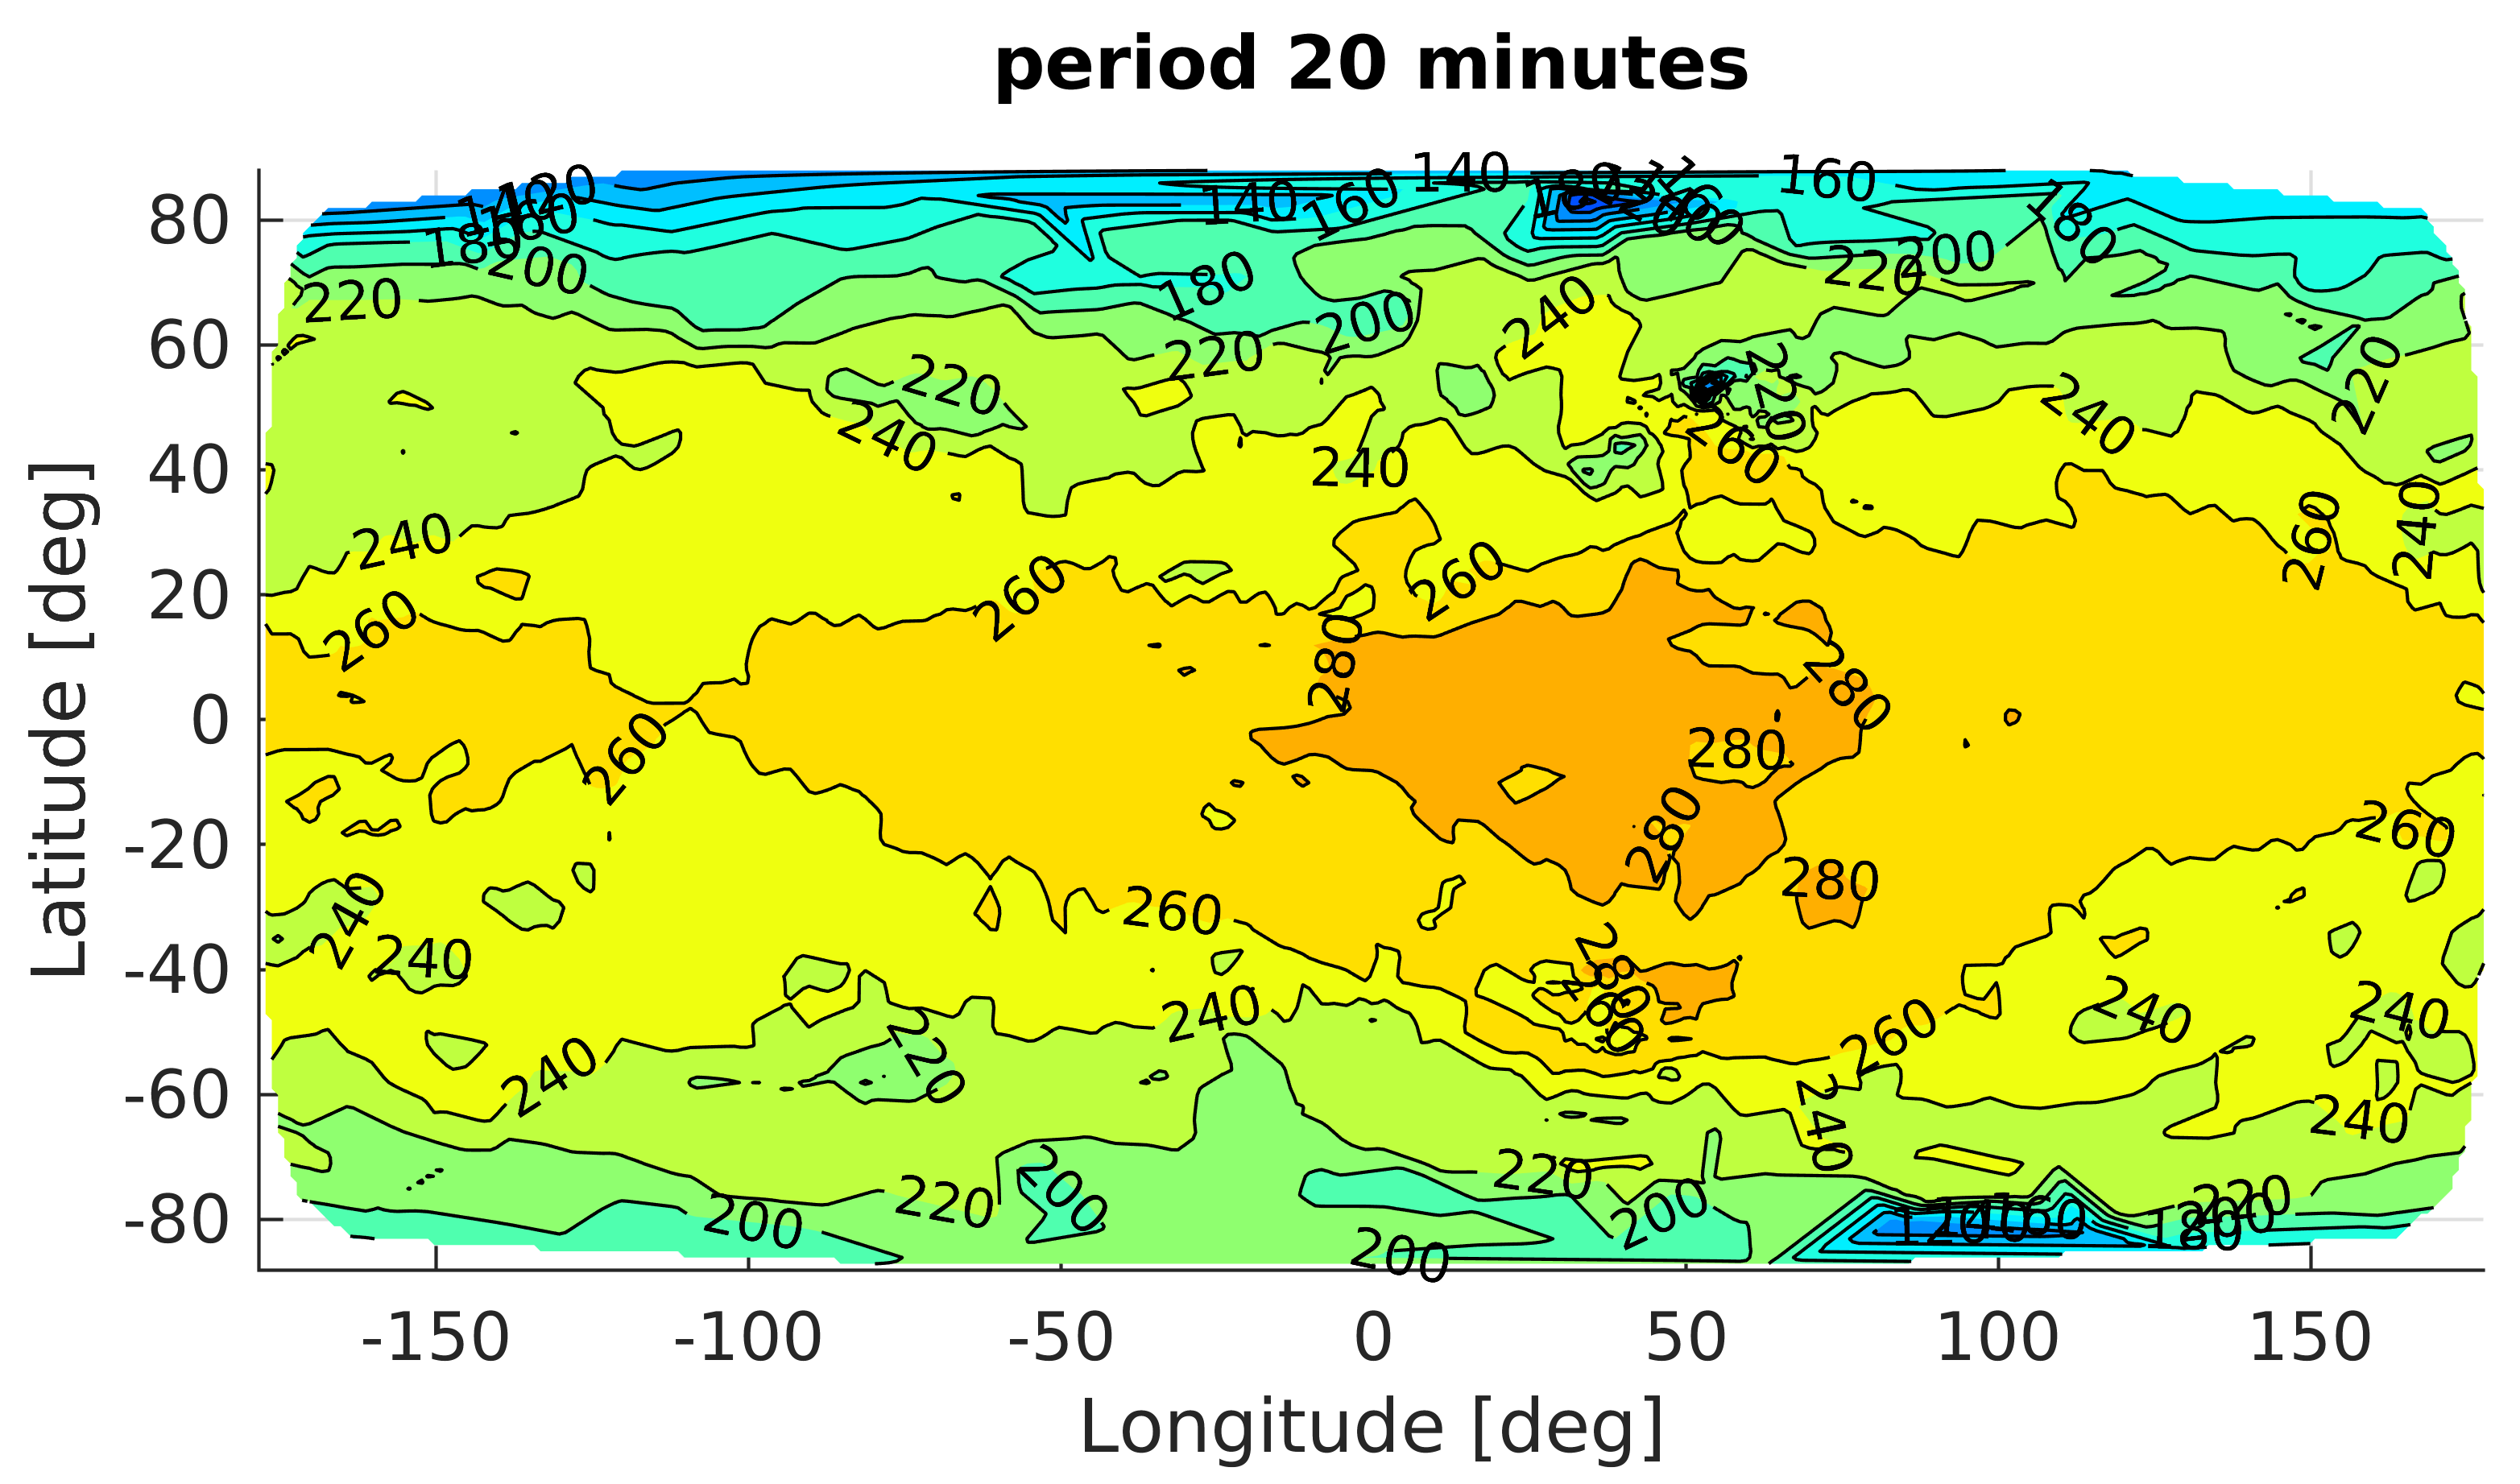
\includegraphics[width=\linewidth]{rsc/theo20mn.png}
    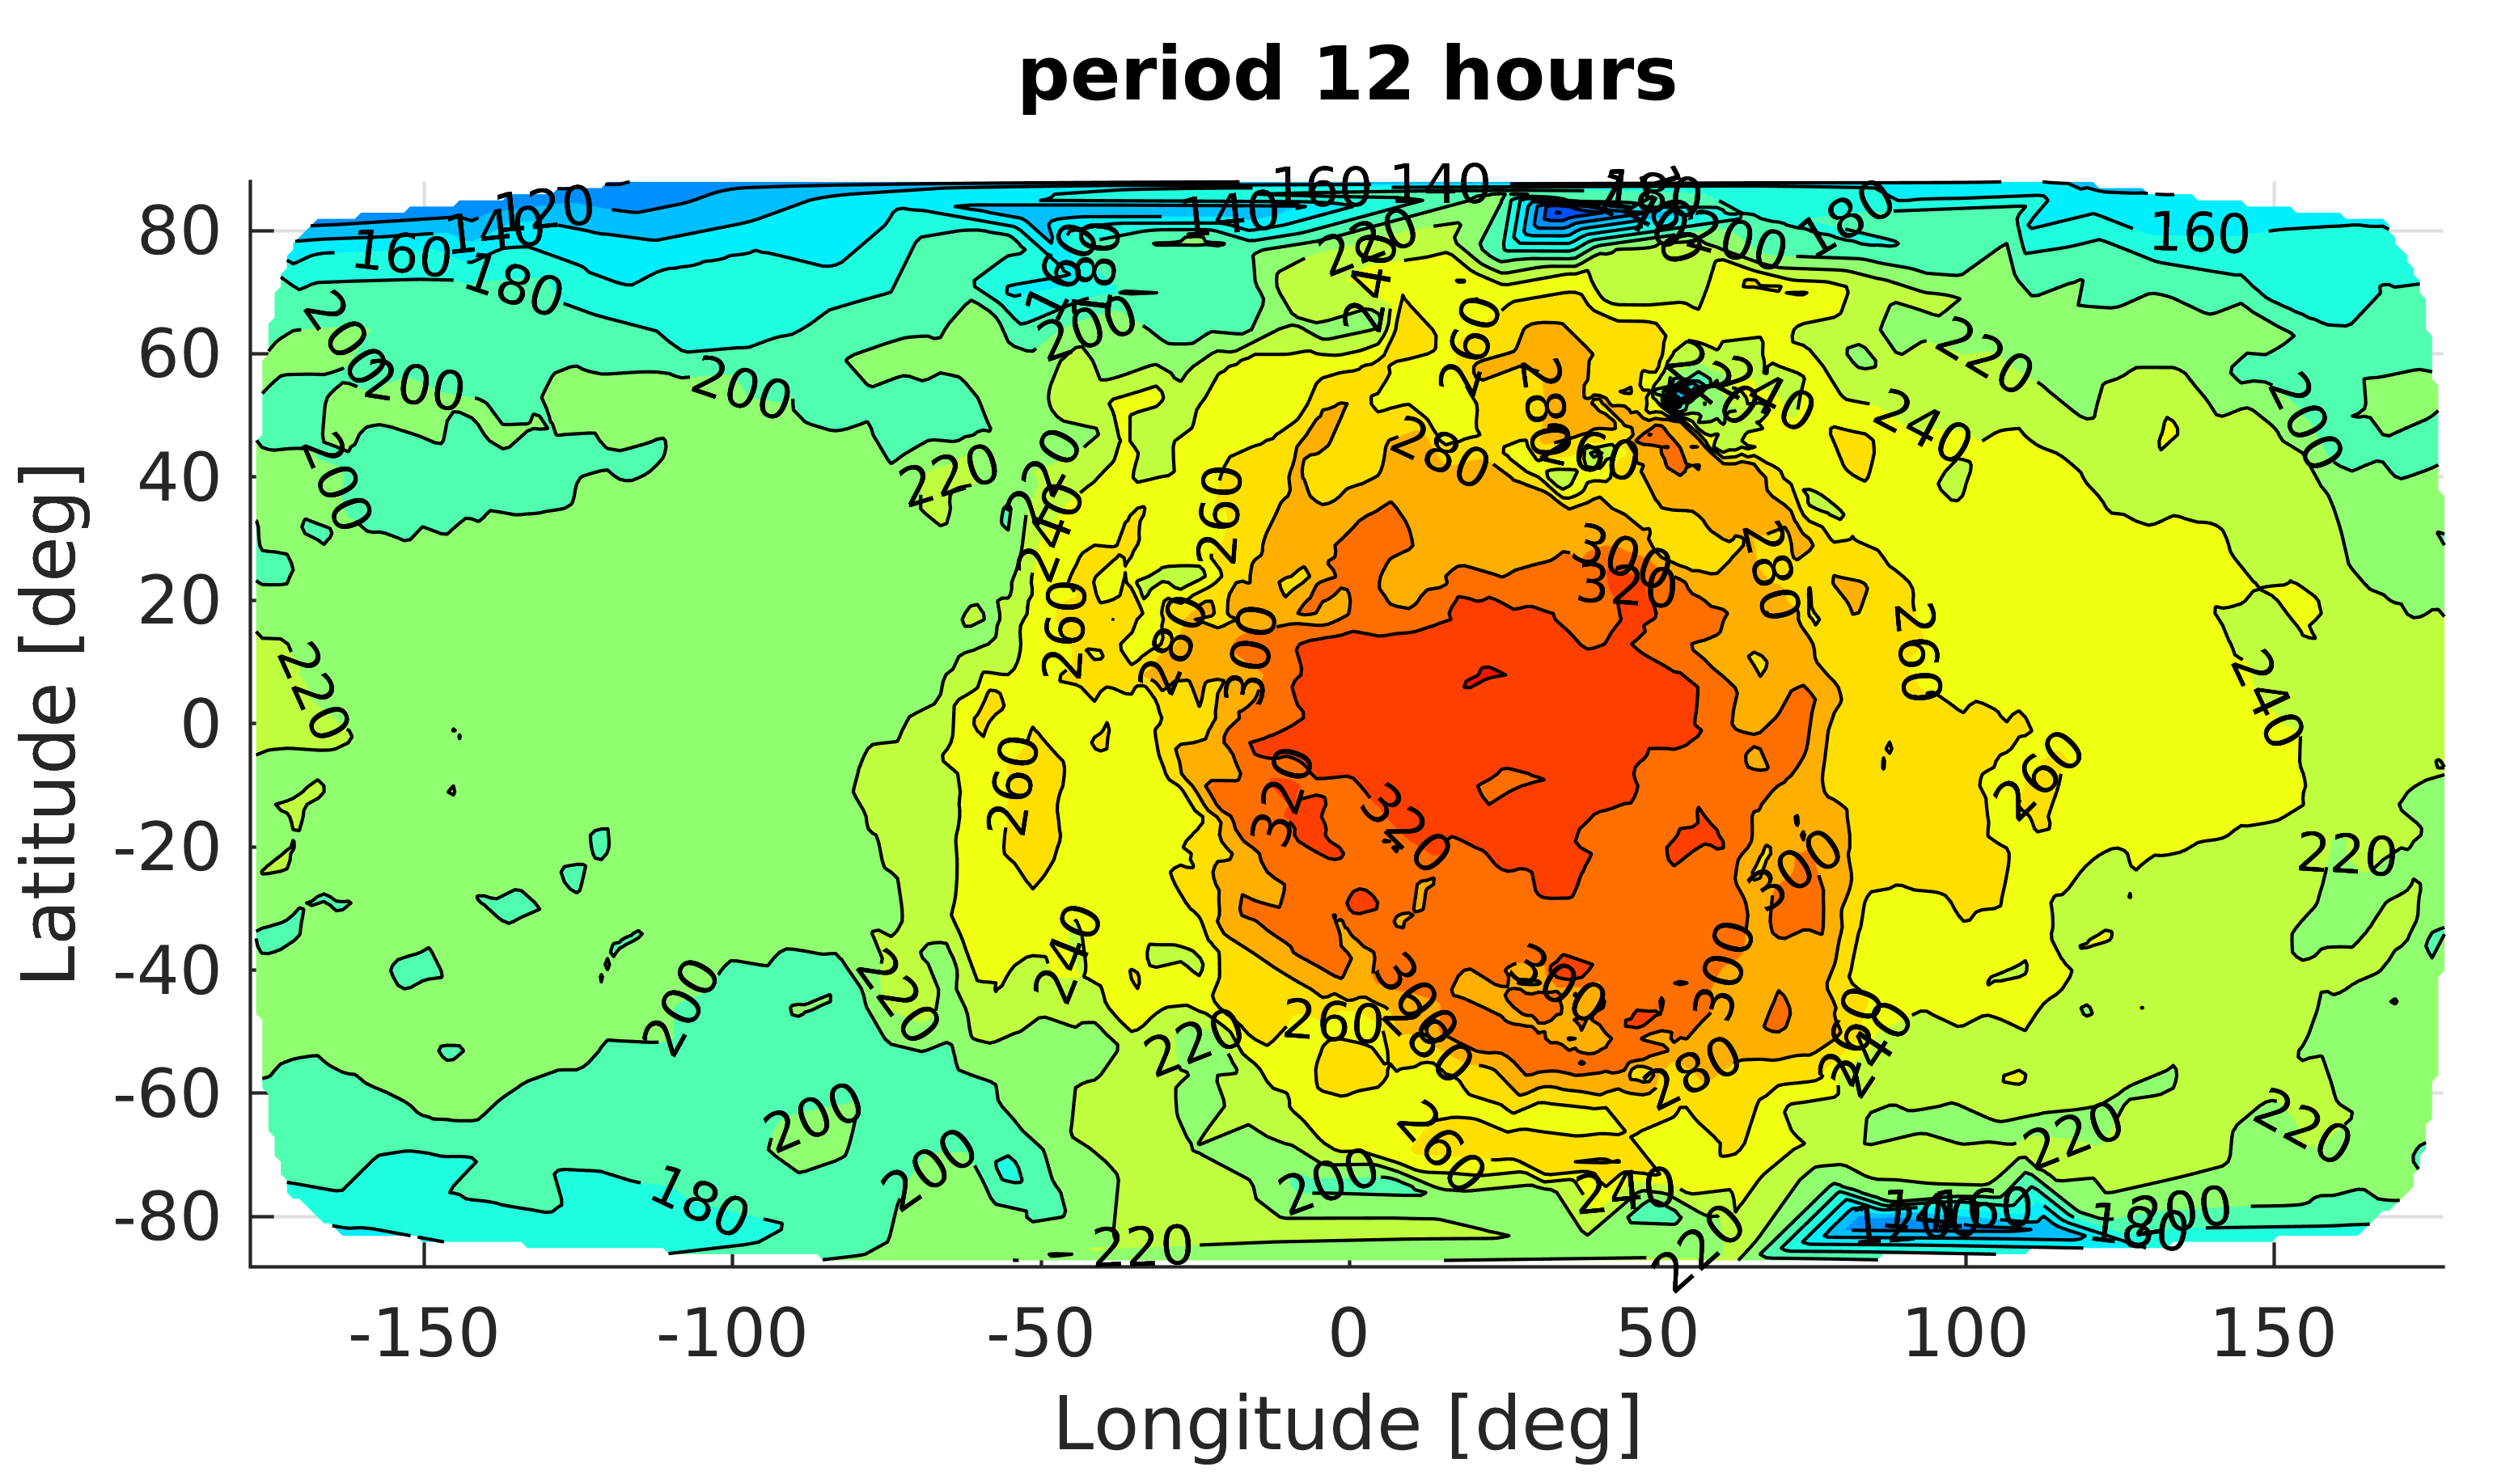
\includegraphics[width=\linewidth]{rsc/theo12h.png}
    \captionof{figure}{Impact of the revolution period of an asteroid on its temperature surface. Every other parameter has been set as in \autoref{sec:4}. The model simply considers \autoref{eq:2.1} without obliquity.}
    \label{fig:7.2}
\end{center}

The difference between the two graphs is the extreme surface temperatures close to the equator. The faster the asteroid rotates, the less extreme the surface temperatures are at midday and midnight. The daily temperature at the equator varies within a range of 120 Kelvins with a revolution period of 12 hours, and only 20 Kelvins with a revolution period of 20 minutes. If the asteroid rotates slower, points on its surface stays longer in the day side and longer in the dark side. For a fast rotating asteroid, the position on the asteroid matters less than for a slow rotating asteroid, as it get less influenced from the Sun orientation toward the position.

\begin{figure*}[t]
    \center
	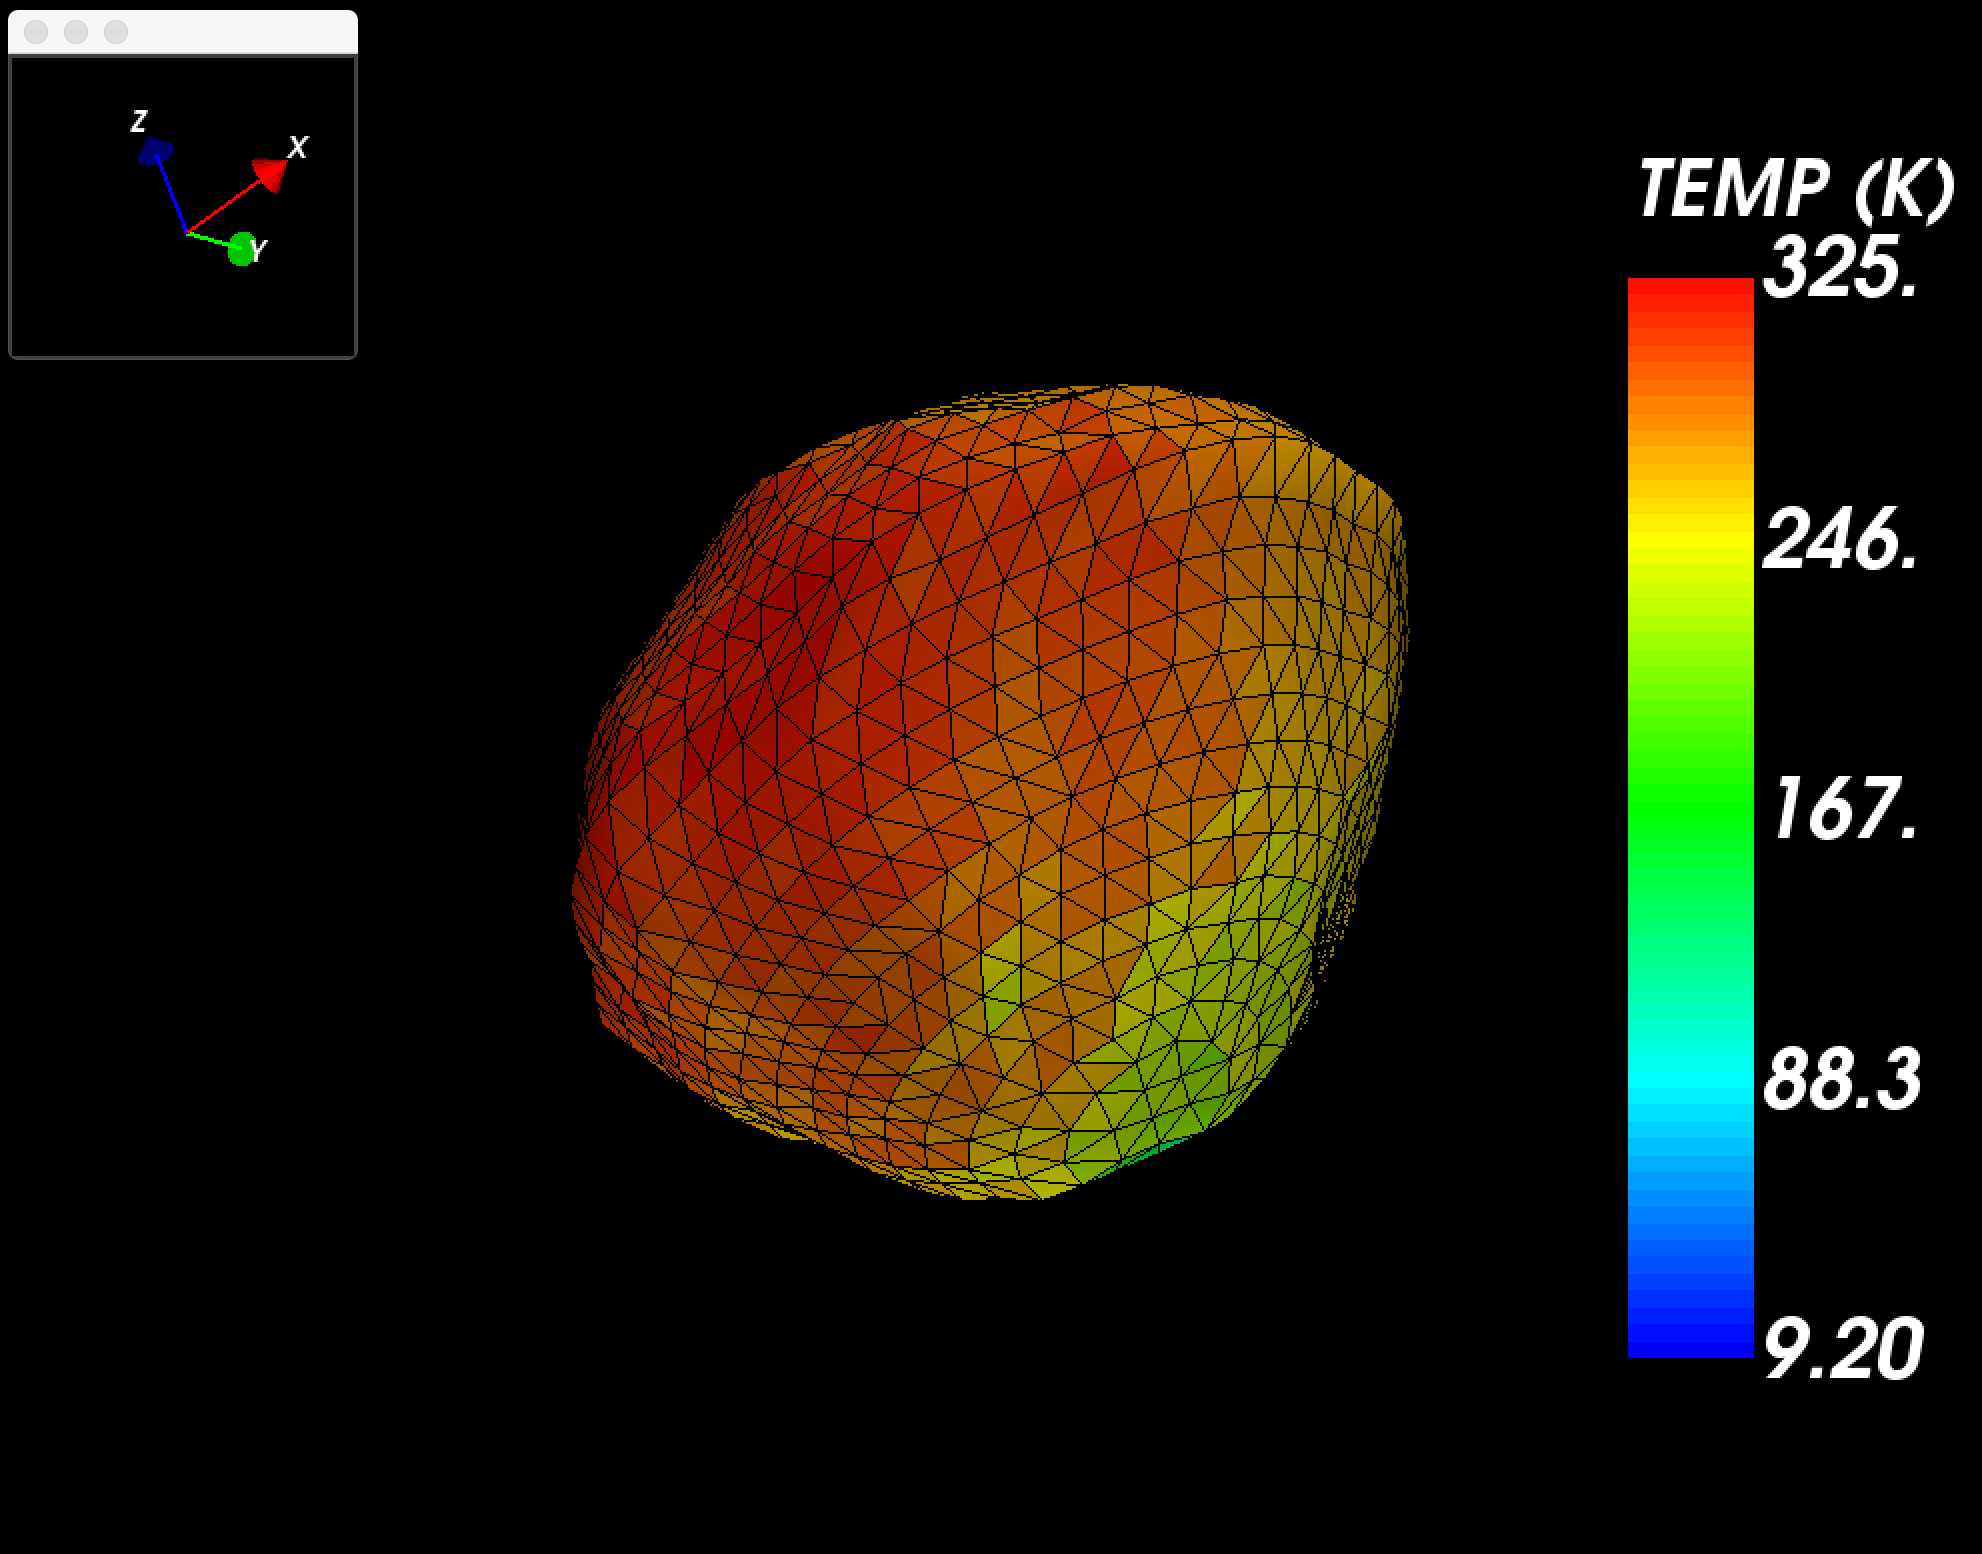
\includegraphics[width=0.3\linewidth]{rsc/HO3_3D_normalspeed}
	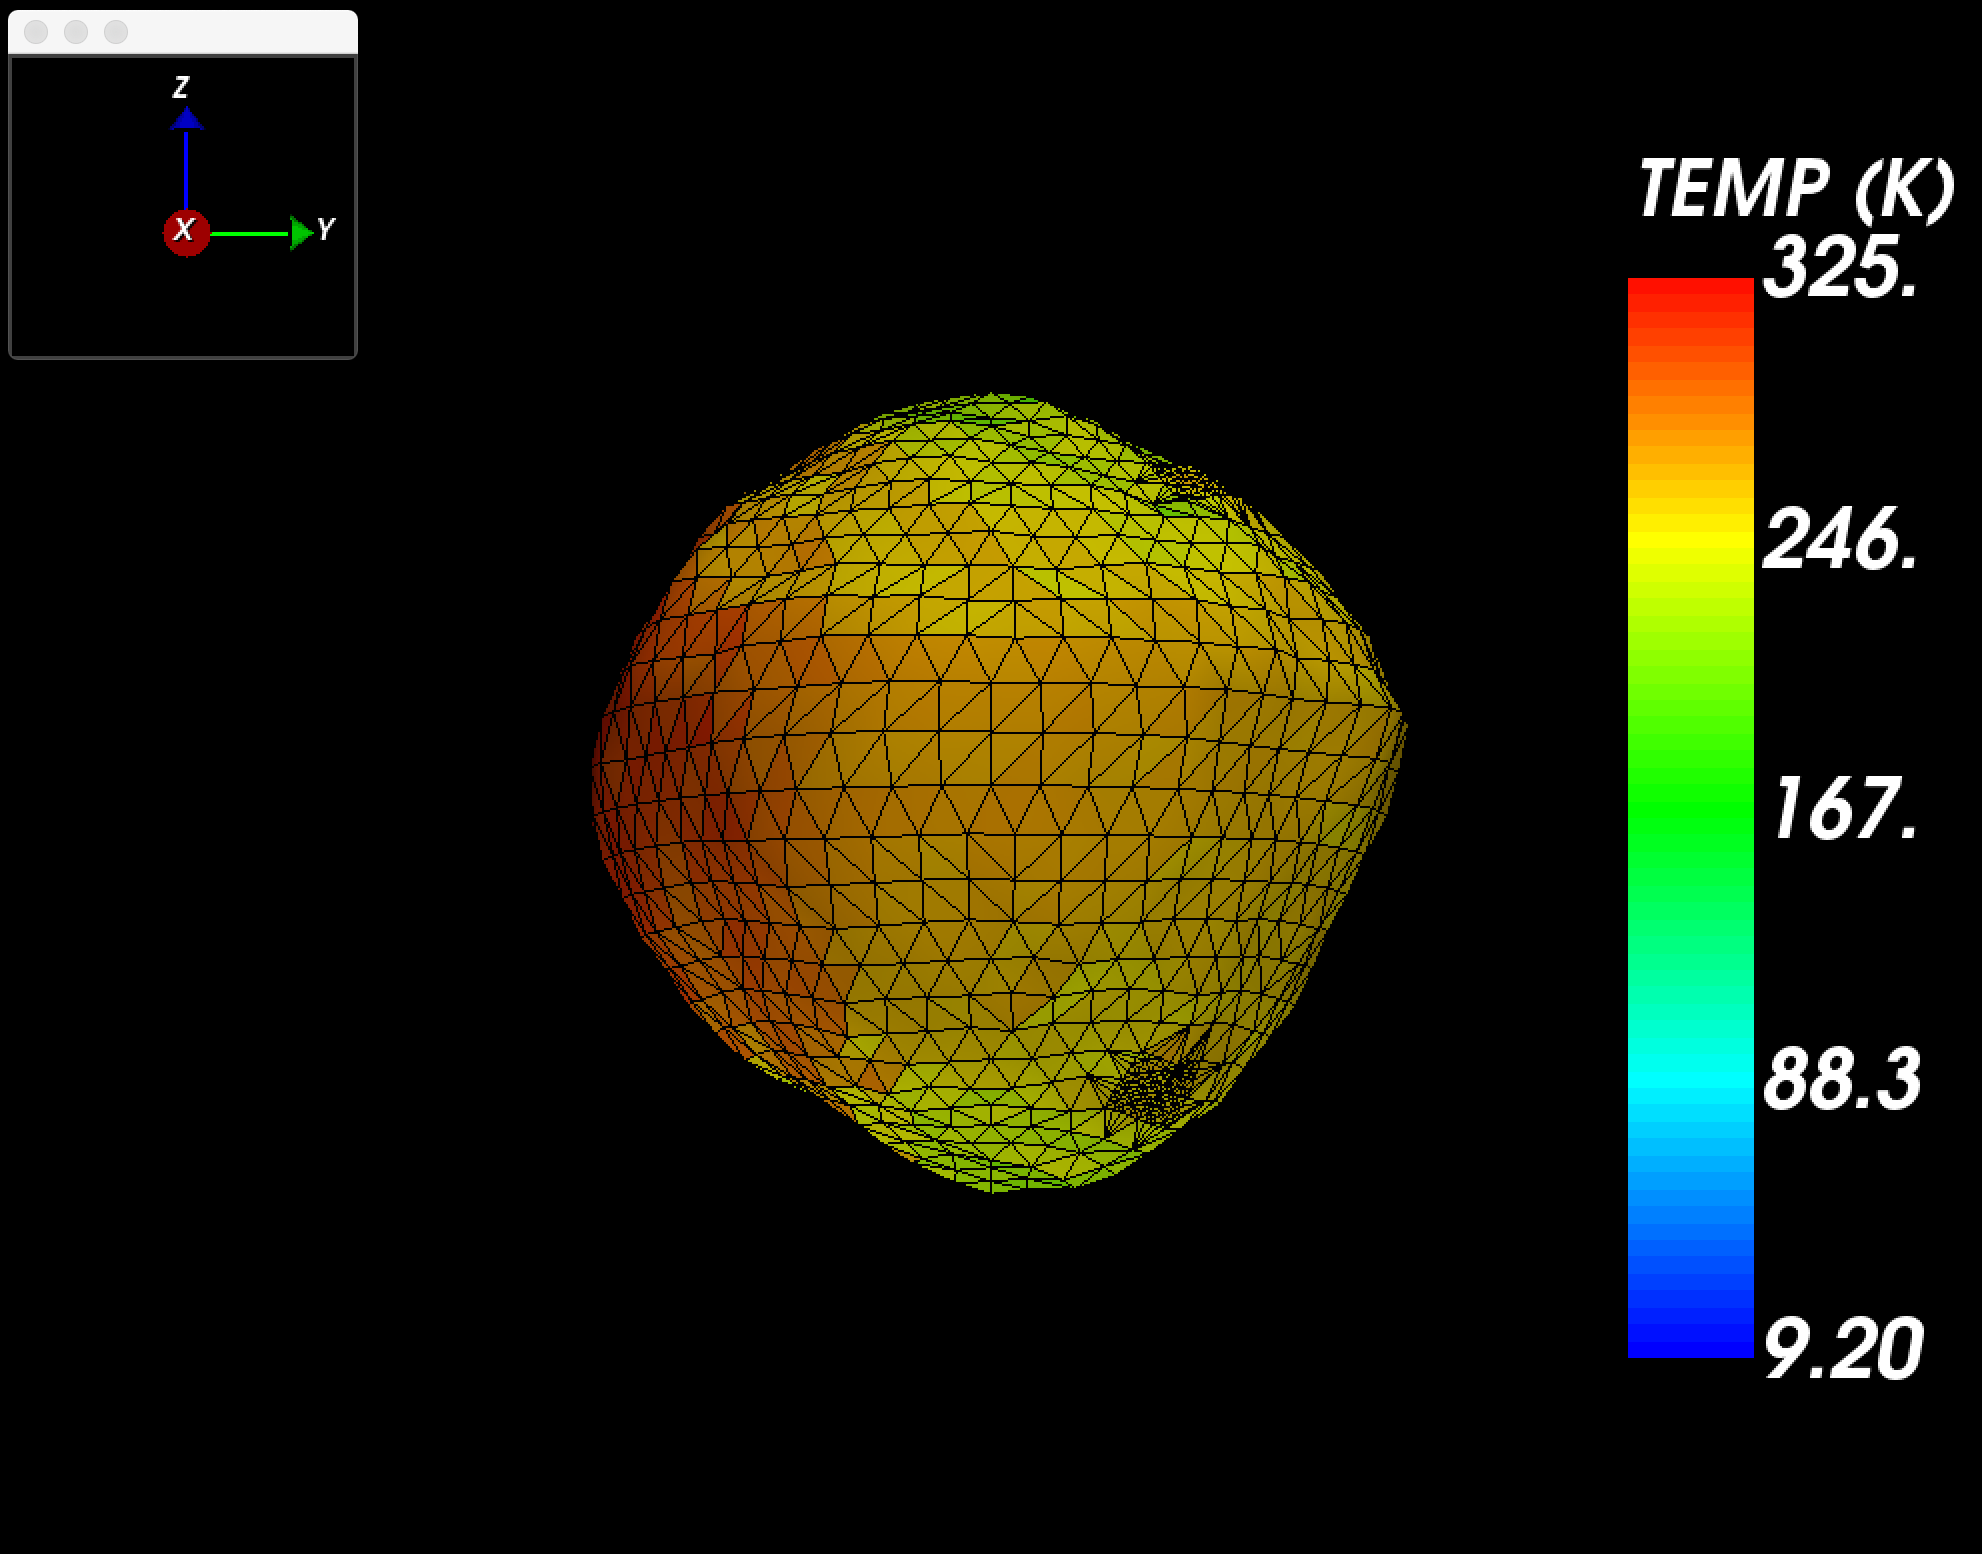
\includegraphics[width=0.3\linewidth]{rsc/HO3_Xaxis_normalspeed}
	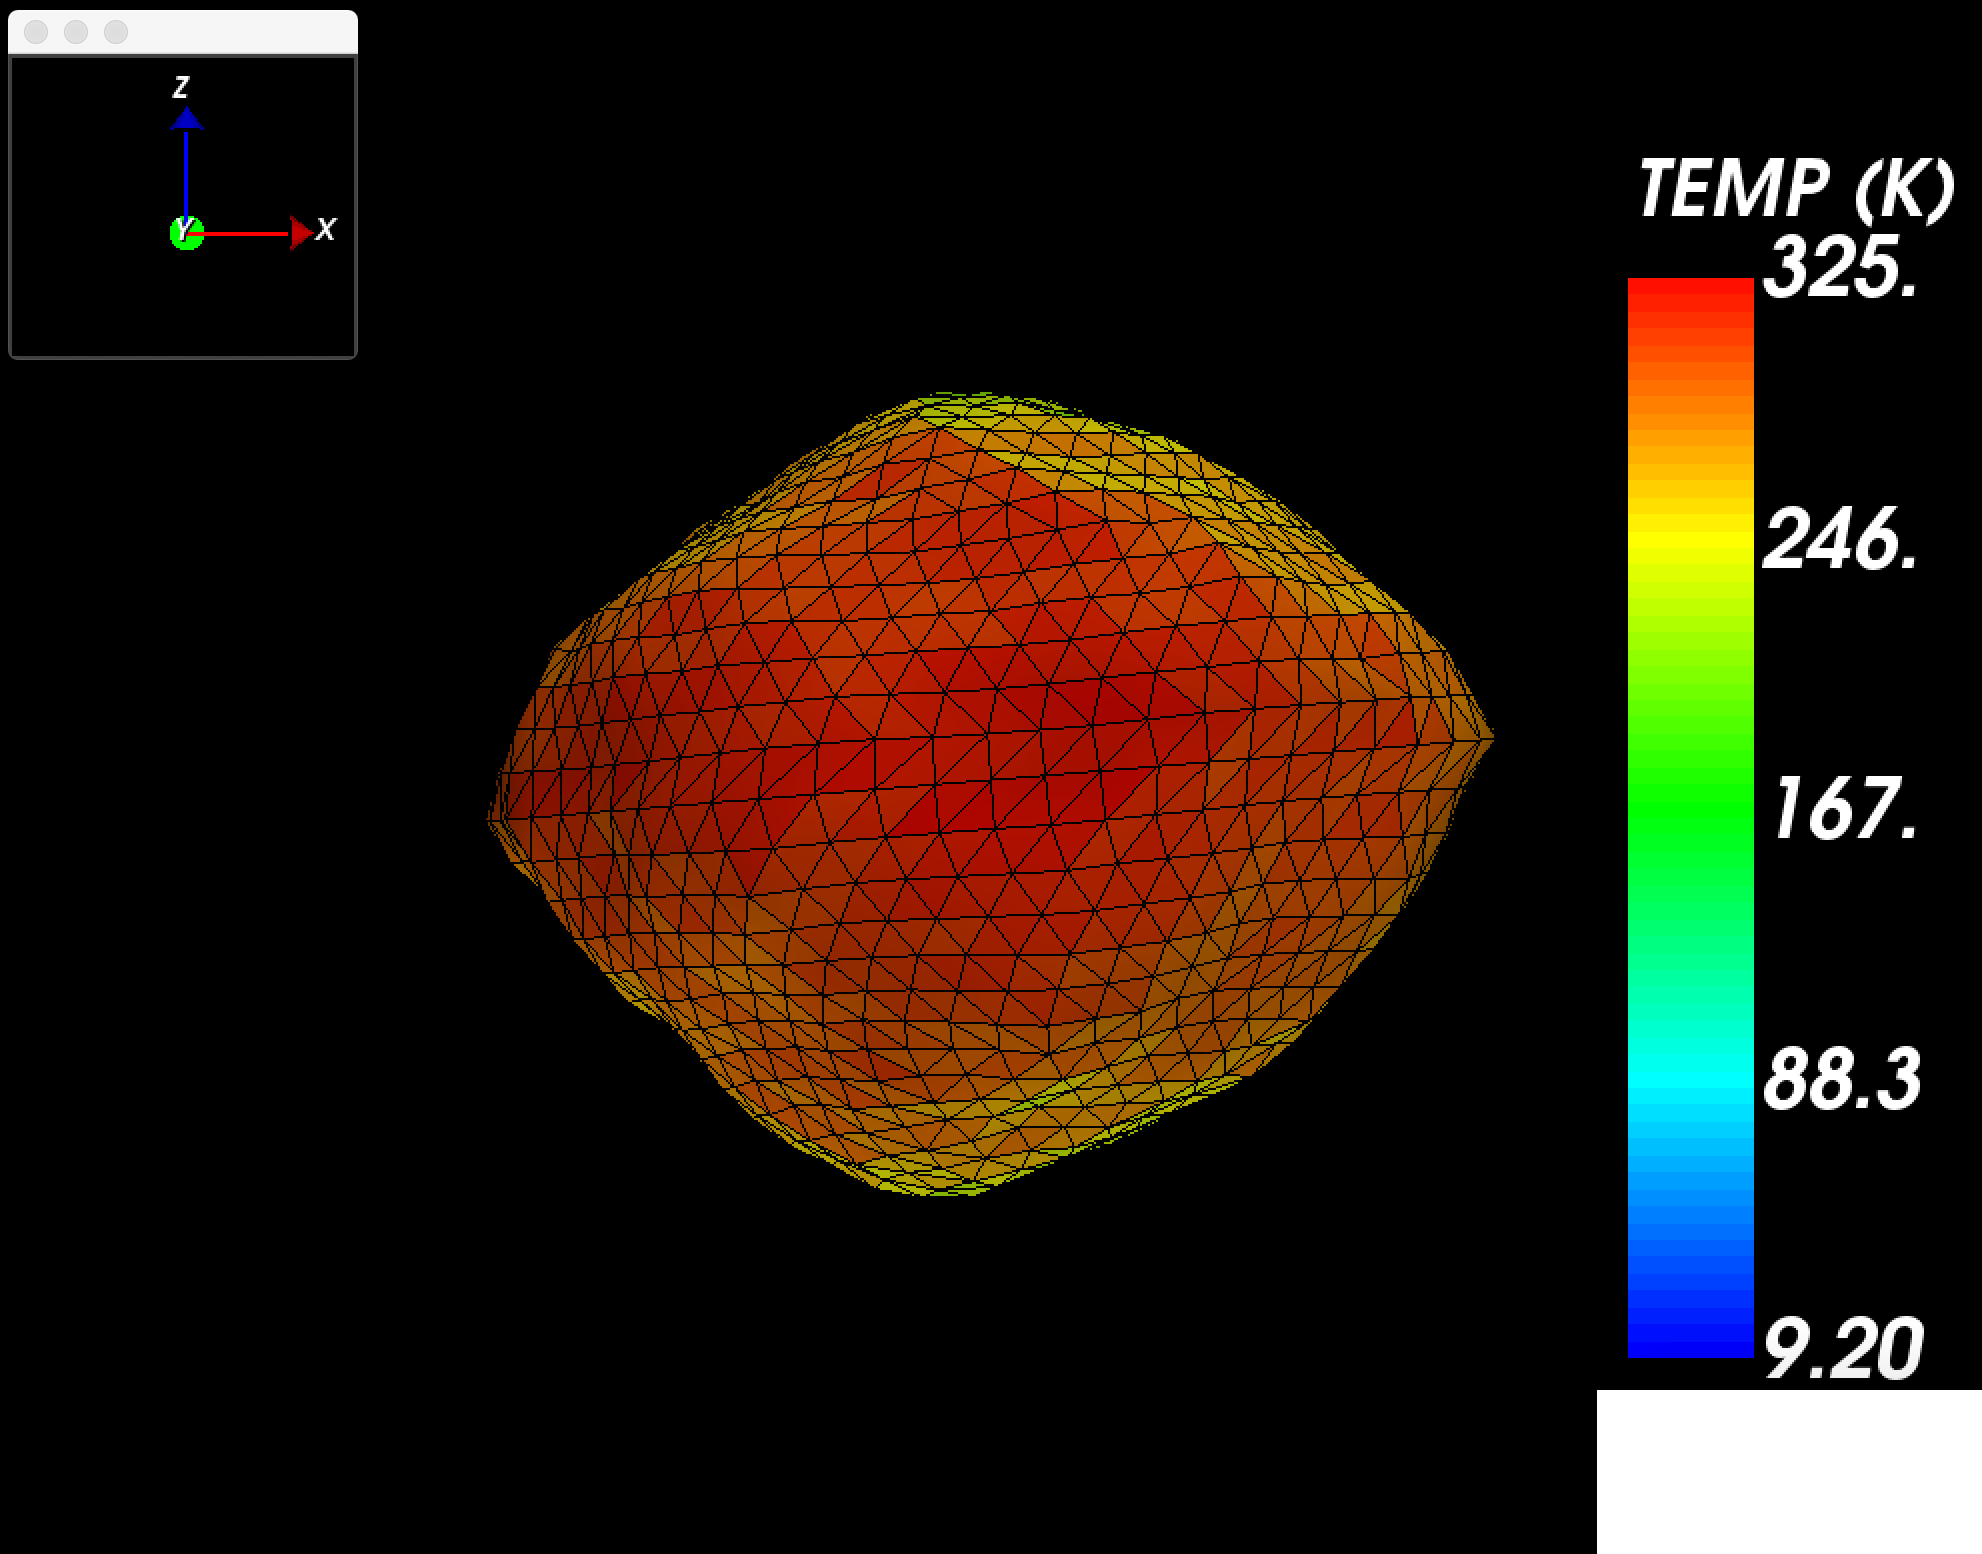
\includegraphics[width=0.3\linewidth]{rsc/HO3_Yaxis_normalspeed}
	\captionof{figure}{Thermal map of the surface temperatures applied on HO3 asteroid's shape model.}
    \label{fig:7.3}
\end{figure*}
